\documentclass[10pt]{article}

\usepackage[margin=0.72in]{geometry}
\usepackage{graphicx}
\usepackage{booktabs}
\usepackage{array}
\usepackage{microtype}
\usepackage{titlesec}
\usepackage{enumitem}

\setlength{\parindent}{0pt}
\setlength{\parskip}{0.35em}
\setlist{nosep}

% Keep headings clearly below the title in size.
\titleformat{\section}
  {\large\bfseries}
  {}
  {0pt}
  {}
\titlespacing*{\section}{0pt}{0.85em}{0.30em}

\titleformat{\subsection}
  {\normalsize\bfseries}
  {}
  {0pt}
  {}
\titlespacing*{\subsection}{0pt}{0.65em}{0.22em}

% Supports compilation either from the repository root or from report/.
\graphicspath{{report/figures/}{figures/}{report/}}

\begin{document}

\begin{center}
    {\Large\bfseries Phase 1: Workload-Dependent GPU/NPU Placement for Edge Vision--Language Inference}\\[0.25em]
    {\small CSE 291A: Systems for LLMs and AI Agents \(\cdot\) Option 2 \(\cdot\) November 4, 2026}
\end{center}

\vspace{-0.4em}

\section{Research Question and Baseline}

\textbf{Question:} When should a vision--language model (VLM) execute visual encoding on the GPU rather than the NPU as request complexity, arrival pattern, and downstream GPU contention change? We optimize end-to-end request latency rather than isolated encoder speed.

Our baseline runs InternVL2-1B INT4 with OpenVINO 2026.1 on a single Intel NUC 16 Pro with a Core Ultra 7 356H. The CPU preprocesses inputs and orchestrates requests. Visual embeddings run on either the GPU or NPU, followed by GPU text embeddings, language prefill, and autoregressive decoding. One GPU language worker handles complete generations serially. Each \(448\times448\) tile contributes 256 visual feature tokens, and we test one, three, and five visual tiles.

\section{Reproducible Workload and Measurements}

The harness captions 40 predecoded video frames reused across requests and records request timestamps, assigned devices, generated tokens, queueing time, stage execution time, and output captions. We vary visual-tile count, text prompt length (11, 107, and 395 tokens), offered arrival rate, and periodic versus irregular arrivals. Irregular interarrival gaps are sampled from an exponential distribution and normalized so that each irregular trace has the same duration and mean arrival rate as its matched periodic trace. Fixed GPU and NPU runs use identical request order and schedules.

Our primary experiment uses three seeds (101, 202, and 303) with 150 requests per placement, arrival pattern, and visual complexity, for 3,600 requests total. Broader Phase 1 profiling covers the placement matrix, rate sweep, prompt-length study, and a short-output sensitivity experiment. We report per-run median and p95 end-to-end latency, throughput, and stage-level queueing and execution time.

\section{Phase 1 Findings}

Isolated encoder speed does not determine the best end-to-end placement. For continuously active single-tile encoding, GPU vision took about 68 ms compared with 94 ms on the NPU. After a 500 ms idle period, these increased to about 84 ms and 158 ms. Controlled background GPU vision traffic also increased GPU language execution from about 154 ms to 254 ms. The main tradeoff is therefore straightforward: GPU vision is faster by itself, but it can compete with downstream language execution for the same accelerator.

Placement changes with workload. GPU-only execution performs well for small inputs and regular, light traffic. As visual complexity and request burstiness increase, NPU offloading becomes more attractive because it moves vision work away from the GPU language stage. At five tiles and roughly 1.97 requests/s, both placements show severe queue buildup, with median latency reaching 28.9 s for GPU-only and 4.91 s with NPU vision.

Prompt length changes the cost of the downstream stage without materially changing vision execution. At 1.5 requests/s with two generated tokens, increasing the text input from 11 to 395 tokens increased internal GPU first-token computation from 56.8 to 141.8 ms for one visual tile and from 158.0 to 247.2 ms for three tiles.

We also tested whether the placement result depends on downstream generation demand. With output capped at two tokens, the irregular-arrival median advantage of NPU offloading became much smaller. For three tiles, GPU/NPU p50 latency changed from 794/675 ms with the original 32-token cap to 598/592 ms. For five tiles, it changed from 1,286/1,014 ms to 948/924 ms. NPU offloading still improved p95 latency. This supports the interpretation that downstream GPU demand is an important reason offloading becomes useful under bursty workloads.

OpenVINO reports execution on GPU.0 and NPU for the corresponding vision paths. Static \(448\times448\) NPU encoding works for both single and sequential multiple tiles. Dynamic-shape compilation and native NPU batches of 2 or 4 failed in the tested runtime, while GPU batches of 2 or 4 were supported but provided little acceleration.

\section{Primary Result: Matched Arrival Patterns}

\begin{figure}[h]
    \centering
    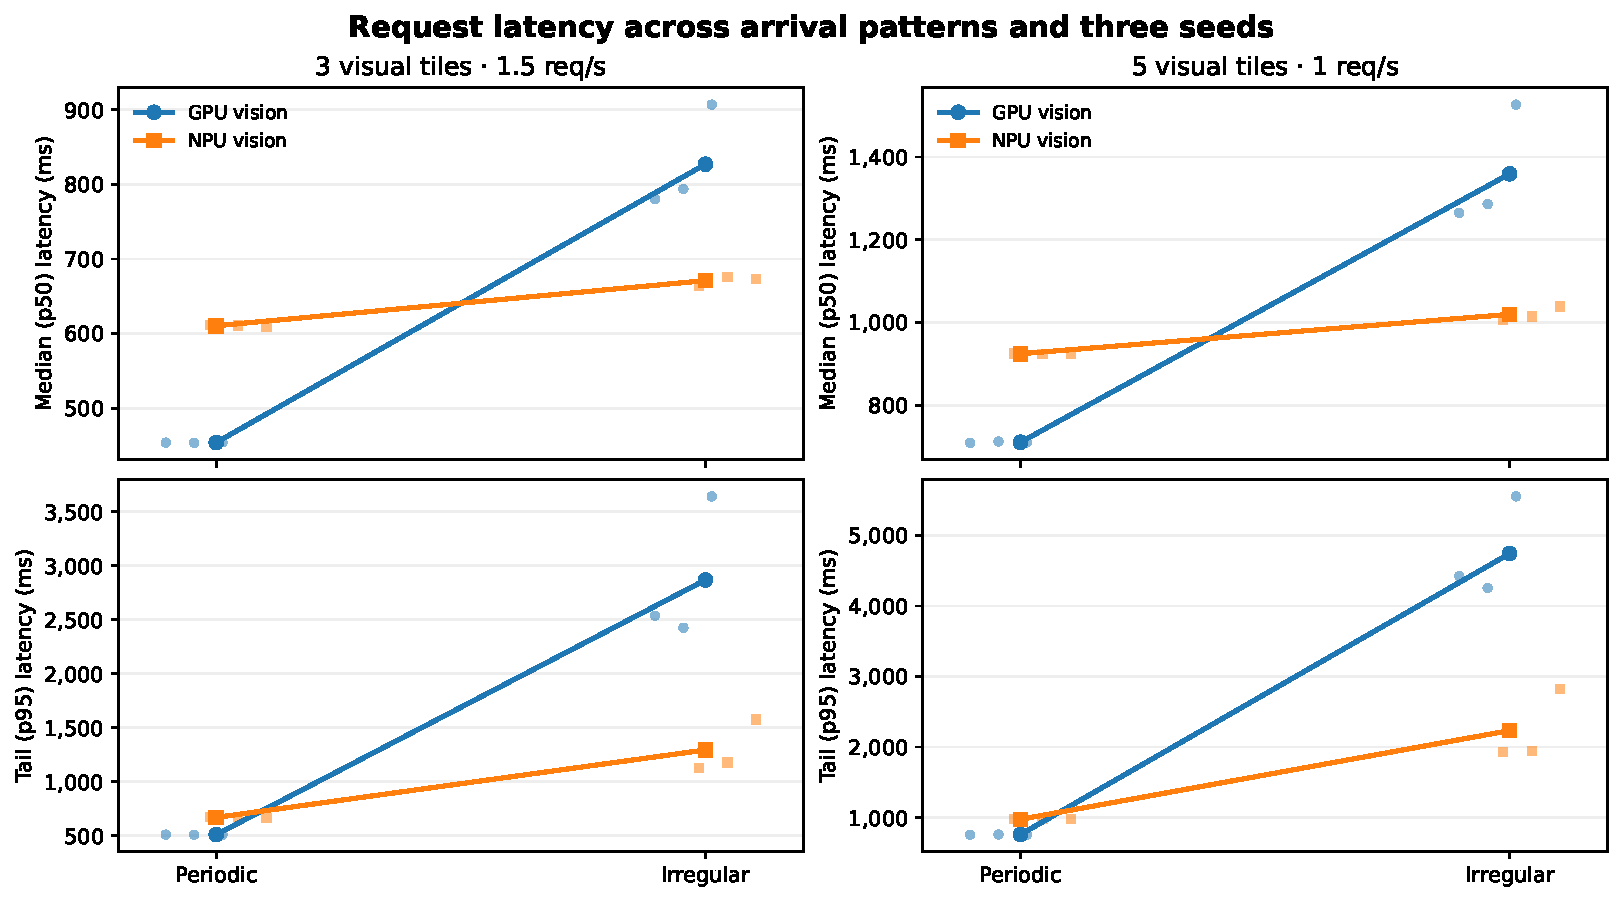
\includegraphics[width=\linewidth]{fig1_placement_reversal_p50_p95.pdf}
    \caption{End-to-end median (top) and p95 (bottom) request latency for matched GPU/NPU workloads. Faint symbols show individual seeds and connected symbols show their means. Three tiles use 1.5 requests/s and five tiles use 1.0 request/s. Periodic and irregular traces have matched mean arrival rates.}
    \label{fig:placement}
\end{figure}

Figure~\ref{fig:placement} shows the clearest placement reversal. In all three seeds and at both visual complexities, GPU vision is faster under periodic arrivals while NPU vision is faster under irregular arrivals. For three tiles, mean run-median latency changes from 454/611 ms for GPU/NPU under periodic traffic to 827/671 ms under irregular traffic. Mean p95 changes from 510/669 ms to 2,869/1,294 ms. For five tiles, median latency changes from 711/925 ms to 1,359/1,020 ms, while p95 changes from 760/977 ms to 4,742/2,234 ms.

The queue measurements explain this reversal. Under periodic traffic, requests rarely wait and the faster GPU encoder wins. Under irregular traffic, GPU-only requests build up primarily before language generation because vision and language share the GPU. NPU offloading moves much of this waiting to the slower but independent vision device, reducing contention at the GPU language stage. The result shows that placement should depend not only on isolated stage latency but also on arrival pattern and downstream resource state.

\section{System Profiles and Key Limitations}

Repeated cached OpenVINO compilation took a median of 1.328 s for GPU vision and 0.104 s for NPU vision. A fresh-process test using a unique cache directory required 1.514 s for GPU vision and 42.127 s for NPU vision. First inference took 79.26 ms and 190.81 ms, followed by warm averages of 67.88 ms and 97.47 ms for GPU and NPU respectively. The full harness in its existing cache state reached tokenizer setup in about 2.9 s and completed frame preprocessing in about 3.7 s.

Maximum host-process RSS increased from roughly 1.3 GiB with one tile to 2.3--2.5 GiB with five tiles. Host-side visual-feature copies, concatenation, and feature insertion were generally small compared with model execution, although GPU embedding calls could become much slower under load.

The main limitations are that the workload reuses only 40 frames and uses a single serialized GPU language worker rather than a production continuous-batching server. GPU and NPU outputs can also differ slightly, so Phase 2 will include an explicit output-quality comparison. Accelerator upload and download costs could not be isolated with the current instrumentation.

\section{Phase 2 Direction}

Phase 2 will develop a lightweight GPU/NPU placement policy using visual-tile count, prompt length, device activity, and stage queues. We will compare it against fixed GPU and NPU placements, simple alternating or queue-aware policies, and the best static placement selected on development workloads. Evaluation will use held-out images and arrival traces and will measure request p50 and p95 latency, throughput, output quality, and scheduling overhead.

\clearpage
\appendix

\section{Timeline and Milestones}

\begin{center}
\begin{tabular}{p{0.18\linewidth} p{0.75\linewidth}}
\toprule
\textbf{Period} & \textbf{Milestone} \\
\midrule
Nov 4  & Complete Phase 1 baseline, measurements, report, and reproducibility package \\
Nov 11 & Finalize workload generation and profiling infrastructure \\
Nov 18 & Complete baseline placement policies \\
Nov 25 & Complete adaptive placement policy and initial ablations \\
Dec 2  & Complete held-out evaluation \\
Dec 9  & Finalize analysis, figures, artifacts, and report \\
Dec 10 & Submit Phase 2 and final report \\
\bottomrule
\end{tabular}
\end{center}

\section{Queueing Mechanism}

\begin{figure}[h]
    \centering
    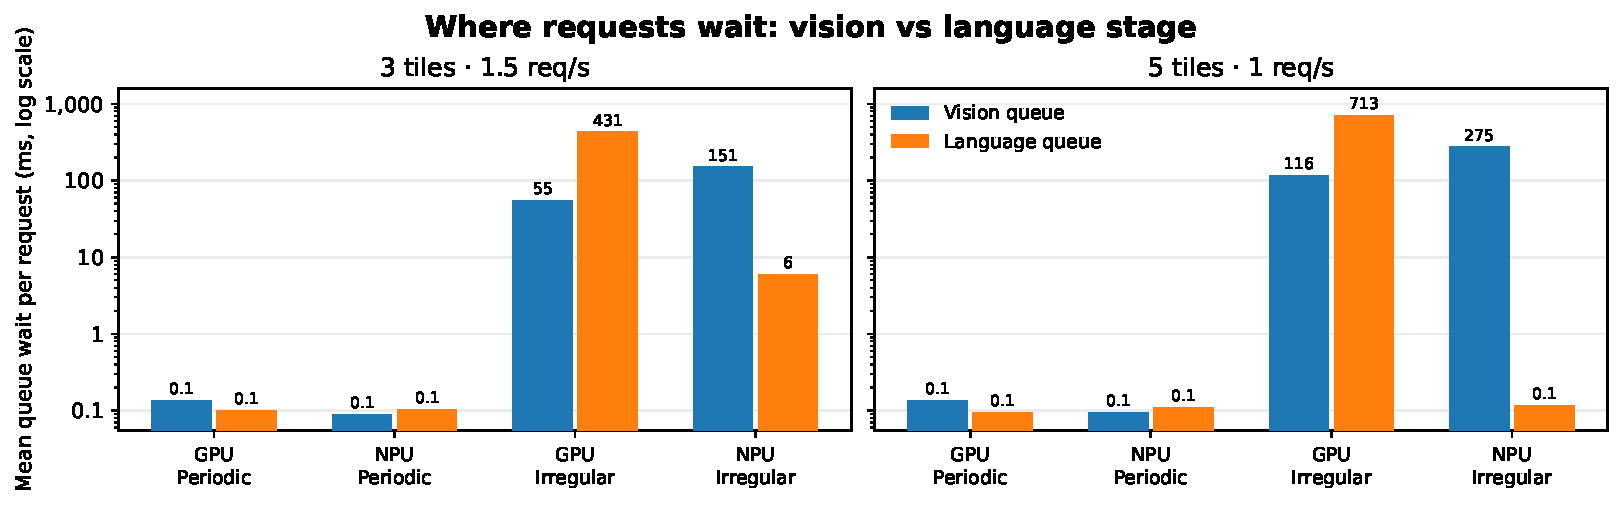
\includegraphics[width=0.93\linewidth]{fig2_queue_wait_log.pdf}
    \caption{Mean vision and language queue wait across three runs on a logarithmic y-axis. Bursty arrivals shift waiting from the GPU language queue toward the NPU vision queue.}
    \label{fig:queues}
\end{figure}

\section{Device Support and Reproducibility}

\begin{center}
\small
\begin{tabular}{p{0.31\linewidth} p{0.18\linewidth} p{0.42\linewidth}}
\toprule
\textbf{Stage / setting} & \textbf{Observed placement} & \textbf{Support} \\
\midrule
Vision encoder, \(448\times448\) & GPU.0, NPU & Both run successfully. NPU requires a static input shape. \\
Vision batch size 2/4 & GPU.0 & GPU supports both sizes with little acceleration. NPU compilation failed in the tested path. \\
Text embeddings & GPU.0 & Verified in the end-to-end benchmark. \\
Language prefill/decode & GPU.0 & Verified with one serialized language worker. \\
Image preparation / queues & CPU host & Python/PIL/NumPy control path. \\
\bottomrule
\end{tabular}
\end{center}

The experiments use Python 3.12.3 and OpenVINO 2026.1.0 on the Intel NUC 16 Pro. The submitted repository includes the Phase 1 workload scripts, figure-generation scripts, curated CSV/log outputs, and environment metadata used for the report. Matched-arrival seeds are 101, 202, and 303. The README documents the input provenance and commands needed to reproduce the reported figures.

\end{document}
